\documentclass[12pt]{extarticle}
%%%%%%%%%%%%%%% PACKAGES %%%%%%%%%%%%%%%
\usepackage{titleps}
\usepackage{url}
\usepackage{amsmath}
\usepackage{cancel}
\usepackage{amsfonts}
\usepackage{amssymb}
\usepackage{mathtools}
\usepackage{graphicx}
\usepackage[dvipsnames]{xcolor}
\usepackage[colorlinks]{hyperref}
\usepackage{geometry}
\geometry{
    a4paper,
    left=19mm,
    right=19mm,
    top=20mm,
    bottom=25mm
}
% Define dark and mid color

\definecolor{Sepia}{HTML}{704214}
\definecolor{RedViolet}{HTML}{C71585}

% Mix lighter shade

\colorlet{LightSepia1}{Sepia!80!yellow}
\colorlet{LightSepia2}{Sepia!70!orange}
\colorlet{DarkGolden}{RedViolet!30!yellow!70!Maroon!70!Brown}
\colorlet{Golden}{RedViolet!30!yellow!70!pink!90!Brown}
\colorlet{DDarkGolden}{RedViolet!20!yellow!70!Maroon!70!Black!65!Brown}

\usepackage{listings}

% Define colors for Visual Studio Code Dark Material them

\definecolor{vscode-bg}{RGB}{30, 30, 30}
\definecolor{vscode-fg}{RGB}{197, 200, 198}
\definecolor{vscode-comment}{RGB}{116, 141, 153}
\definecolor{vscode-purple}{RGB}{198, 120, 221}
\definecolor{vscode-green}{RGB}{86, 156, 214}

% Define style for Python cod

\lstdefinestyle{mystyle}{
    backgroundcolor=\color{vscode-bg},
    basicstyle=\color{vscode-fg}\footnotesize\ttfamily, % Set font to Fira Code
    commentstyle=\color{vscode-comment},
    keywordstyle=\color{vscode-purple},
    stringstyle=\color{vscode-green},
    numberstyle=\tiny\color{vscode-fg},
    tabsize=2,
    showlines=false, % Remove white grid between lines
}

% Set Python language for syntax highlighting
\lstset{style=mystyle, language=Python}
%%%%%%%%%%%%%%%%%%%%%%%%%%%%%%%%%%%%%%%%
%%%%%%%%%%%%%%% FONT %%%%%%%%%%%%%%%%%%%
\usepackage[T1]{fontenc}
\usepackage{charter}

\def\primarycolor{DarkGolden}
\def\secondarycolor{Golden}
%%%%%%%%%%%%%%%%%%%%%%%%%%%%%%%%%%%%%%%%
%%%%%%%%%%%%%%% HEADER %%%%%%%%%%%%%%%%%
\usepackage{fancyhdr}
\let\oldheadrule\headrule
\renewcommand{\headrule}{\color{\secondarycolor}\oldheadrule}
\renewcommand{\headrulewidth}{0.7pt}
\pagestyle{fancy}
\fancyhead{}\fancyfoot{}
\fancyhead[L]{\scshape \large \color{\primarycolor}{\fontfamily{qpl}\selectfont
Amirreza "Farnam" Taheri \\
Student ID: 4021300198003
}}
\fancyhead[R]{\color{\secondarycolor} Game Theory}
\fancyfoot[C]{\textcolor{\primarycolor}{(\thepage)}}
\setlength{\headheight}{1cm}

\fancypagestyle{headerpage}{
    \fancyhf{} % Clear header and footer
    \renewcommand{\headrulewidth}{0pt} % Remove header rule
    \renewcommand{\footrulewidth}{0pt} % Remove footer rule
    \fancyhead[R]{} % Remove the line that displays "Course Name (Course Code)" in the header page
}

%%%%%%%%%%%%%%%%%%%%%%%%%%%%%%%%%%%%%%%%
%%%%%%%%%%%%%%% COMMANDS %%%%%%%%%%%%%%%
% \newcommand{\norm}[1]{\lVert#1\rVert}
% \newcommand{\inner}[1]{\langle#1\rangle}
\newcommand{\problem}[1]{
    \subsection*{\textcolor{\secondarycolor}{#1}}
    \addcontentsline{toc}{subsection}{\protect\numberline{}#1}
}
\newcommand{\partof}[1]{
    \subsubsection*{\textcolor{\secondarycolor}{(#1)}}
    \addcontentsline{toc}{subsubsection}{\protect\numberline{}#1}
}
%%%%%%%%%%%%%%%%%%%%%%%%%%%%%%%%%%%%%%%%
%%%%%%%%%%%%%%% BODY %%%%%%%%%%%%%%%%%%%
\linespread{1.4}
\color{DDarkGolden}
\begin{document}
\setlength{\abovedisplayskip}{6pt}
\setlength{\belowdisplayskip}{6pt}
\setlength{\abovedisplayshortskip}{0pt}
\setlength{\belowdisplayshortskip}{0pt}
%%%%%%%%%%%%%%% CONTENT %%%%%%%%%%%%%%%%
\thispagestyle{headerpage} % Apply custom header style to this page only
\begin{center}
    \vspace*{1.5cm}
    {\Huge\bfseries\color{\primarycolor}{\fontfamily{qpl}\selectfont Exercise 2}} \\
    \vspace{3cm}
    
\includegraphics[width=6cm]{teias.png} \\ % Replace "university_logo.png" with the actual filename of your university logo
    \vspace{2cm}
    {\Large\color{\primarycolor}{\fontfamily{qpl}\selectfont Amirreza "Farnam" Taheri}} \\
    {\large\color{\primarycolor}{Student ID: 4021300198003}} \\
    \vspace{3cm}
    {\large\bfseries\color{\secondarycolor}{Macroeconomics I}} \\
    \vspace{1cm}
    {\large\color{\secondarycolor}{Instructor: Prof. Hosein Joshaghani}} \\
    \vspace{3cm}
    {\large\color{\secondarycolor}{March 11, 2024}} % Replace with the actual date or semester information
\end{center}
\newpage % Add a page break after the header page

%%%%%%%%%%%%%%% CONTENT %%%%%%%%%%%%%%%%
\pagestyle{fancy} % Apply fancy header to the remaining pages
\fancyhead[R]{\color{\secondarycolor} Problemset 2} % Display "Problemset #no" in the header of the remaining pages
%%%%%%%%%%%%%%%%%%%%%%%%%%%%%%%%%%%%%%%%
%%%%%%%%%%%%%%%%%%%%%%%%%%%%%%%%%%%%%%%%
\textbf{\Large\begin{center}
    {Analytical Study}
\end{center}}
\problem{a.}What are the steady-state values of physical capital, human capital, and output, all per unit of effective
labor?\\\\
We have:
\begin{itemize}
    \item \begin{math}
        Y=K^\alpha \;H^\beta\; (AL)^{1-\alpha-\beta}
    \end{math}
    \item \begin{math}
        \dot k = S_K k^\alpha h^\beta-(g+n+\delta)k
    \end{math}
    \item \begin{math}
        \dot h = S_H k^\alpha h^\beta-(g+n+\delta)k
    \end{math}
\end{itemize}
In the fix point, the system has no dynamic, so we have:\\
\begin{align*}
    \dot k &= 0\\
    S_Kk^\alpha h^\beta-(g+n+\delta)k&=0\\
    S_Kk^\alpha h^\beta&=(g+n+\delta)k\\
    k^{\alpha-1}&=(g+n+\delta)h^{-\beta}S_K^{-1}\\
    k^*&=(\dfrac{h^{*\beta} S_K}{g+n+\delta})^{\frac{1}{1-\alpha}}\;\star\\
\end{align*}
\begin{align*}
    \dot h &= 0\\
    S_H k^\alpha h^\beta-(g+n+\delta)h&=0\\
    S_H k^\alpha h^\beta&=(g+n+\delta)h\\
    h^{\beta-1}&=(g+n+\delta)k^{-\alpha}S_K^{-1}\\
    h^*&=(\dfrac{k^{*\beta} S_K}{g+n+\delta})^{\frac{1}{1-\beta}}\;\star\star\\
\end{align*}
We also have:
\begin{align*}
    S_Kk^\alpha h^\beta&=(g+n+\delta)k\\
    S_Hk^\alpha h^\beta&=(g+n+\delta)h\\
    \xRightarrow{Divide}\;\dfrac{S_K}{S_H}&=\dfrac{k}{h}\\
    \implies \;h^*&=\dfrac{S_H}{S_K}k^*\;\star\star\:\star\\\\
\end{align*}
%%%%%%%%%%%%%%%%%%%%%%%%%%%%%%%%%%%%%%%%
By substituting $\star\star\star$ in $\star$, we would have:\\
\begin{align*}
    k^*&=\;(\dfrac{(\dfrac{S_H}{S_K}k^*)^{\beta} S_K}{g+n+\delta})^{\frac{1}{1-\alpha}}\\
    &=\;k^{*\beta}(\dfrac{{S_H}^{\beta} S_K^{1-\beta}}{g+n+\delta})^{\frac{1}{1-\alpha}}\\\\
    \implies k^*& =\; \{(\dfrac{{S_H}^{\beta} S_K^{1-\beta}}{g+n+\delta})^{\frac{1}{1-\beta-\alpha}} \;\lor\; 0\}\\\\
\end{align*}
By substituting $\star\star\star$ in $\star\star$, we would have:\\
\begin{align*}
    h^*&=\;(\dfrac{(\dfrac{S_K}{S_H}h^*)^{\alpha} S_H}{g+n+\delta})^{\frac{1}{1-\beta}}\\
    &=\;(\dfrac{h^{*\alpha} {S_K}^{\alpha} S_H^{1-\alpha}}{g+n+\delta})^{\frac{1}{1-\beta}}\\\\
    \implies h^*& =\; \{(\dfrac{{S_K}^{\alpha} S_H^{1-\alpha}}{g+n+\delta})^{\frac{1}{1-\alpha-\beta}} \;\lor\; 0\}\\
\end{align*}
\newpage
%%%%%%%%%%%%%%%%%%%%%%%%%%%%%%%%%%%%%%%%
%%%%%%%%%%%%%%%%%%%%%%%%%%%%%%%%%%%%%%%%
\problem{b.}What is the growth rate of output per capita in steady state?\\\\\\
We know that the output per effective labor has no Dynamic at the fix point.
Output per capita equals to output per effective labor times productivity. So at the fix point, it grows with rate of productivity growth wich is equal to "$n$".

\newpage
%%%%%%%%%%%%%%%%%%%%%%%%%%%%%%%%%%%%%%%%
%%%%%%%%%%%%%%%%%%%%%%%%%%%%%%%%%%%%%%%%
\problem{c.}Study the effect of changes in $s_h$ and $s_k$ on steady state values of $y, k, h$.\\\\\\\\
At fixed point, we have:
\begin{align*}
    h&=(\dfrac{{S_K}^{\alpha} S_H^{1-\alpha}}{g+n+\delta})\\
\end{align*}
So by taking derivative, we would have:
\begin{align*}
    \dfrac{\partial k}{\partial S_H}&=\dfrac{(1-\alpha)(\dfrac{{S_H}^{1-\alpha} S_K^{\alpha}}{g+n+\delta})^{\frac{1}{1-\beta-\alpha}}}{S_H(1-a-b)}\\
    \dfrac{\partial k}{\partial S_K}&=\dfrac{\alpha(\dfrac{{S_H}^{1-\alpha} S_K^{\alpha}}{g+n+\delta})^{\frac{1}{1-\beta-\alpha}}}{S_K(1-a-b)}\\\\\\\\
\end{align*}
%%%%%%%%%%%%%%%%%%%%%%%%%%%%%%%%%%%%%%%%
At fixed point, we have:
\begin{align*}
    k&= (\dfrac{{S_H}^{\beta} S_K^{1-\beta}}{g+n+\delta})^{\frac{1}{1-\beta-\alpha}}\\
\end{align*}
So by taking derivative, we would have:
\begin{align*}
    \dfrac{\partial k}{\partial S_H}&=\dfrac{\beta(\dfrac{{S_H}^{\beta} S_K^{1-\beta}}{g+n+\delta})^{\frac{1}{1-\beta-\alpha}}}{S_H(1-a-b)}\\
    \dfrac{\partial k}{\partial S_K}&=\dfrac{(1-\beta)(\dfrac{{S_H}^{\beta} S_K^{1-\beta}}{g+n+\delta})^{\frac{1}{1-\beta-\alpha}}}{S_K(1-a-b)}
\end{align*}
\newpage
%%%%%%%%%%%%%%%%%%%%%%%%%%%%%%%%%%%%%%%%
At fixed point, we have:
\begin{align*}
    y&=(\dfrac{S_{H}^{\beta} S_K^{1-\beta}}{g+n+\delta})^{\frac{\alpha}{1-\beta-\alpha}}(\dfrac{S_{H}^{\alpha} S_K^{1-\alpha}}{g+n+\delta})^{\frac{\beta}{1-\alpha-\beta}}\\
    &=(\dfrac{S_K}{g+n+\delta})^{\frac{\alpha}{1-\beta-\alpha}}(\dfrac{{S_H}}{g+n+\delta})^{\frac{\beta}{1-\alpha-\beta}}\\
\end{align*}
So by taking derivative, we would have:
\begin{align*}
    \dfrac{\partial y}{\partial S_H}=-\dfrac{\beta(\dfrac{S_K}{g+n+\delta})^{\frac{\alpha}{1-\beta-\alpha}}(\dfrac{{S_H}}{g+n+\delta})^{\frac{\beta}{1-\alpha-\beta}}}{S_H(\alpha+\beta-1)}\\
    \dfrac{\partial y}{\partial S_K}=-\dfrac{\alpha(\dfrac{S_K}{g+n+\delta})^{\frac{\alpha}{1-\beta-\alpha}}(\dfrac{{S_H}}{g+n+\delta})^{\frac{\beta}{1-\alpha-\beta}}}{S_K(\alpha+\beta-1)}\\
\end{align*}
\newpage
%%%%%%%%%%%%%%%%%%%%%%%%%%%%%%%%%%%%%%%%
%%%%%%%%%%%%%%%%%%%%%%%%%%%%%%%%%%%%%%%%
\problem{d.}Linearize the system around the non-trivial fixed point, and find the Eigenvalues associated with it.\\
\textbf{Bonus:} Do they represent the convergence rate in the proximity of the fixed point? If the answer is
negative, try finding the convergence rates.\\\\\\
To linearize the system around the non-trivial fixed point,
we need to set up the Jacobian matrix and find the Eigenvalues.\\\\
We had the following system of differential equations:
\begin{align*}
    \dot{k} &= S_K k^\alpha h^\beta - (g + n + \delta)k \\
    \dot{h} &= S_H k^\alpha h^\beta - (g + n + \delta)h
\end{align*}\\
The Jacobian matrix at the fixed point $(k^*, h^*)$ is:
$$J = \begin{bmatrix}
    \frac{\partial \dot{k}}{\partial k} & \frac{\partial \dot{k}}{\partial h} \\
    \frac{\partial \dot{h}}{\partial k} & \frac{\partial \dot{h}}{\partial h}
\end{bmatrix}_{(k^*, h^*)}$$\\\\
Now we should calculate the partial derivatives, to set up the Jacobian matrix:\\
\begin{align*}
    \frac{\partial \dot{k}}{\partial k} &= \alpha S_K {k^*}^{\alpha-1} {h^*}^\beta - (g + n + \delta) \\
    \frac{\partial \dot{k}}{\partial h} &= \beta S_K {k^*}^\alpha {h^*}^{\beta-1} \\
    \frac{\partial \dot{h}}{\partial k} &= \alpha S_H {k^*}^{\alpha-1} {h^*}^\beta \\
    \frac{\partial \dot{h}}{\partial h} &= \beta S_H {k^*}^\alpha {h^*}^{\beta-1} - (g + n + \delta)
\end{align*}
\newpage
%%%%%%%%%%%%%%%%%%%%%%%%%%%%%%%%%%%%%%%%
To find the eigenvalues, we must solve the following equation:\\
$$\det(J - \lambda I) = 0$$\\
$$\det\begin{bmatrix*}
    \alpha S_K {k^*}^{\alpha-1} {h^*}^\beta - (g + n + \delta)-\lambda && \beta S_K {k^*}^\alpha {h^*}^{\beta-1}\\
    \alpha S_H {k^*}^{\alpha-1} {h^*}^\beta && \beta S_H {k^*}^\alpha {h^*}^{\beta-1} - (g + n + \delta)-\lambda
\end{bmatrix*}=0$$\\\\
By calculating the determinant, we will reach to the following equation:
\begin{align*}
    -(g + n + \delta +\lambda)\left[\alpha S_K {k^*}^{\alpha-1} {h^*}^\beta +\beta S_H {k^*}^\alpha {h^*}^{\beta-1} - (g + n + \delta + \lambda)^2\right]&=0
\end{align*}
\begin{align*}
    (i)\;&g + n + \delta +\lambda=0\;\\
    \implies\; &\lambda = -(g + n + \delta)\;\;\checkmark
\end{align*}
\begin{align*}
    (ii)\;&\alpha S_K {k^*}^{\alpha-1} {h^*}^\beta +\beta S_H {k^*}^\alpha {h^*}^{\beta-1} - (g + n + \delta + \lambda)^2=0\\
    \implies\;&\lambda=\sqrt{\alpha S_K {k^*}^{\alpha-1} {h^*}^\beta +\beta S_H {k^*}^\alpha {h^*}^{\beta-1}}-g-n-\delta\;\;\checkmark
\end{align*}
%%%%%%%%%%%%%%%%%%%%%%%%%%%%%%%%%%%%%%%%
%%%%%%%%%%%%%%%%%%%%%%%%%%%%%%%%%%%%%%%%
\newpage
\textbf{\large\begin{center}
    {Quantitaive Analysis}
\end{center}}
\problem{e.}Plot the phase diagram of the system in $h-k$ plane by hand.\\\\\\
\begin{figure*}[h!]
    \centering
    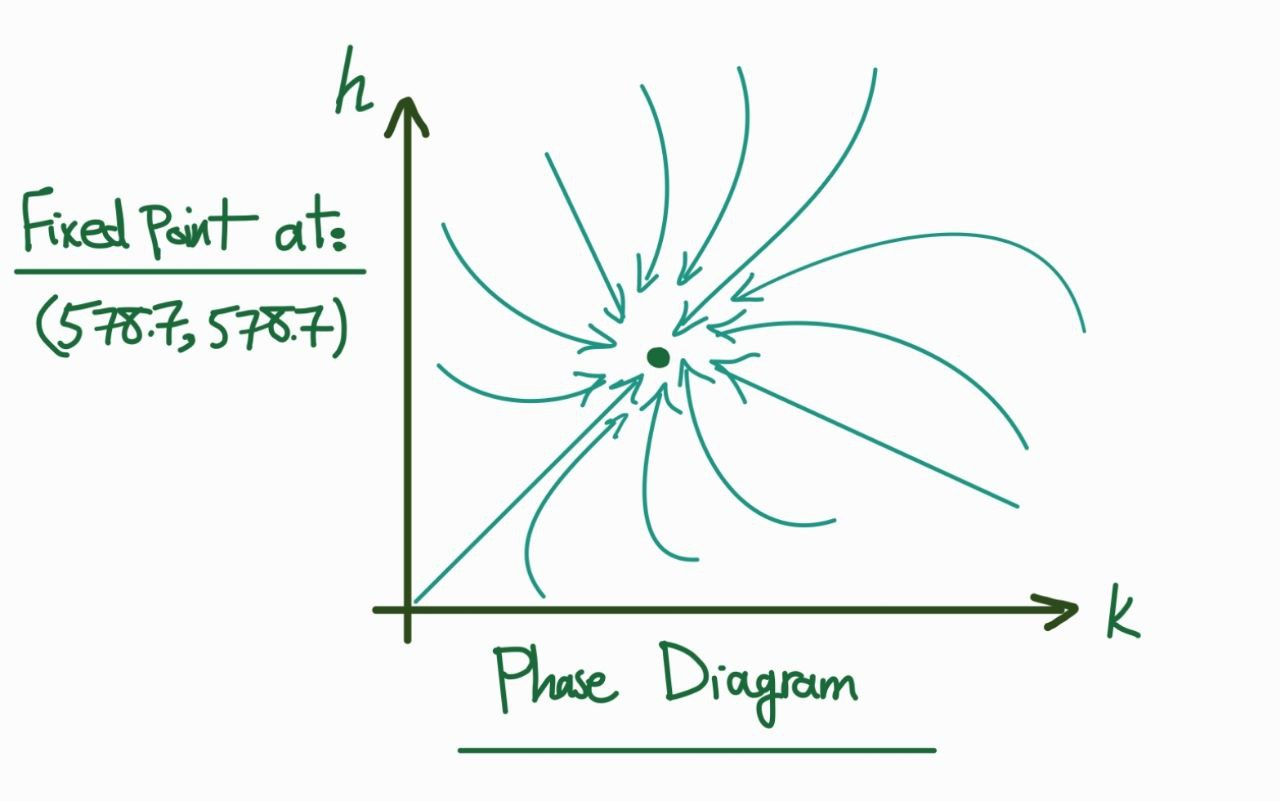
\includegraphics[width=15cm]{Phase Diagram Hand.jpg}
\end{figure*}
\newpage
%%%%%%%%%%%%%%%%%%%%%%%%%%%%%%%%%%%%%%%%
\problem{f.}Plot the phase diagram of the system in $h-k$ plane using Matlab or Python. (Solve the system using
ODE45).\\\\
\begin{center}
    \large\textbf{To open the python code for this problem: \href{run:f - Phase plot.ipynb}{Click Here}}\\
\end{center}
\begin{figure*}[h!]
    \centering
    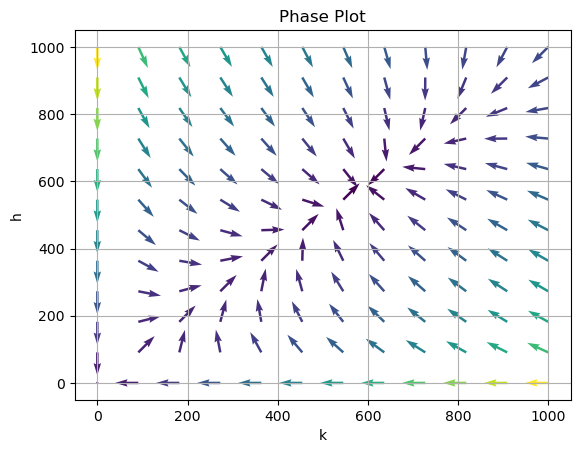
\includegraphics[width=11.5cm]{phase_plot_ODE.png}
\end{figure*}
\begin{figure*}[h!]
    \centering
    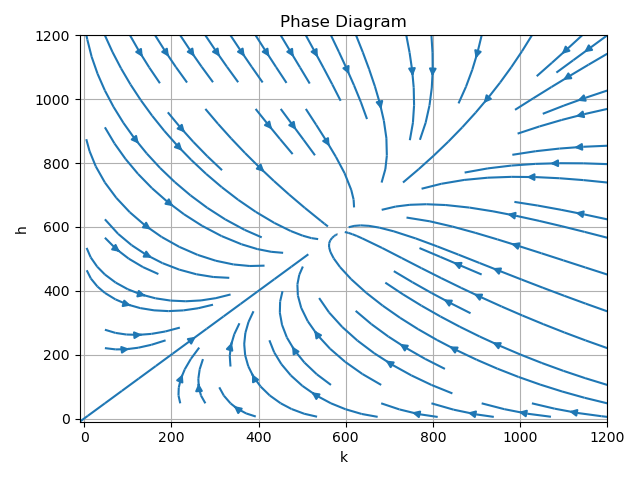
\includegraphics[width=12cm]{phase_diagram_stream.png}
\end{figure*}
\newpage
%%%%%%%%%%%%%%%%%%%%%%%%%%%%%%%%%%%%%%%%
\problem{g.}Choose any arbitrary initial condition, close to non-trivial fixed point of the system, and plot the transient
responses for $k, h, y$.\\\\\\
\begin{center}
    \large\textbf{To open the python code for this problem: \href{run:g - Transient Plot.ipynb}{Click Here}}\\
\end{center}
\vspace*{1cm}
\begin{figure*}[h!]
    \centering
    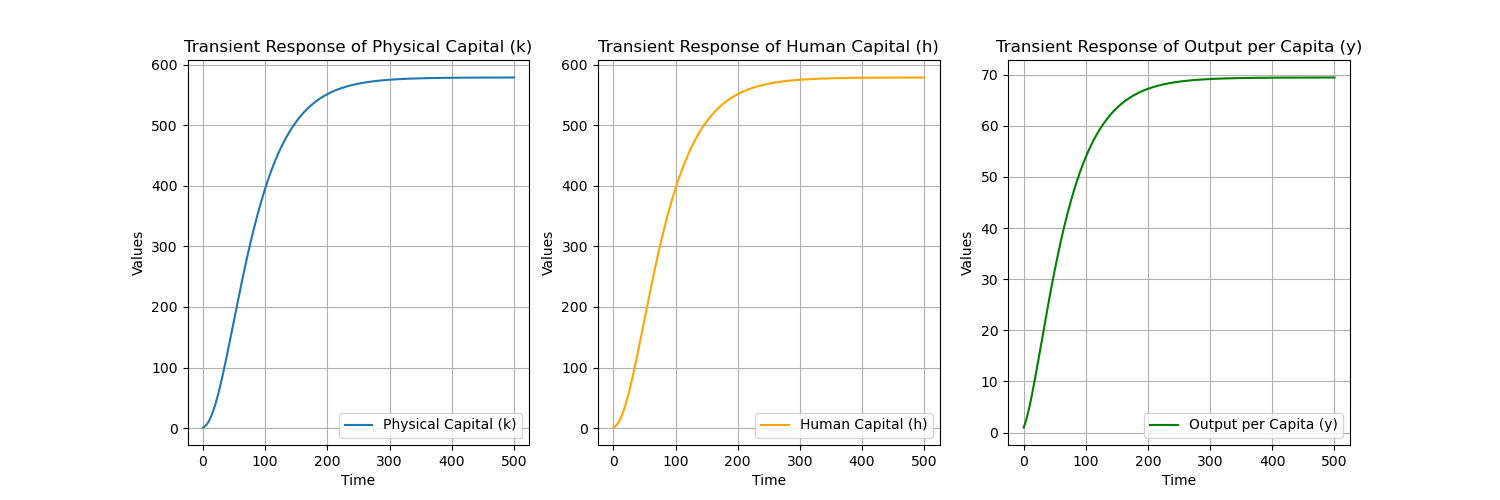
\includegraphics[width=19cm]{transient_response_plot.png}
\end{figure*}
\newpage
%%%%%%%%%%%%%%%%%%%%%%%%%%%%%%%%%%%%%%%%
\problem{h.}Write the equations of motion obtained in part (a) in discrete time. Use “Dynare” to solve the system
numerically, and compare your results.\\
\begin{center}
    \large\textbf{To open the Dynare code for this problem: \href{run:Farnam.mod}{Click Here}}
\end{center}
\begin{figure*}[h!]
    \centering
    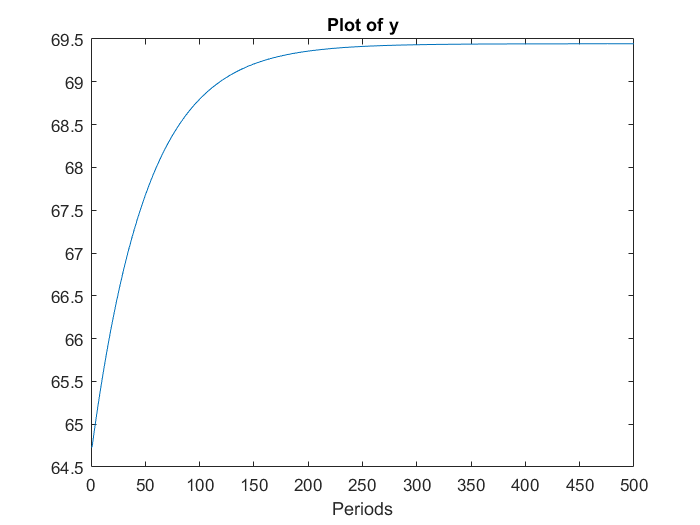
\includegraphics[width=8cm]{y-simulated.png}
\end{figure*}
\begin{figure*}[h!]
    \centering
    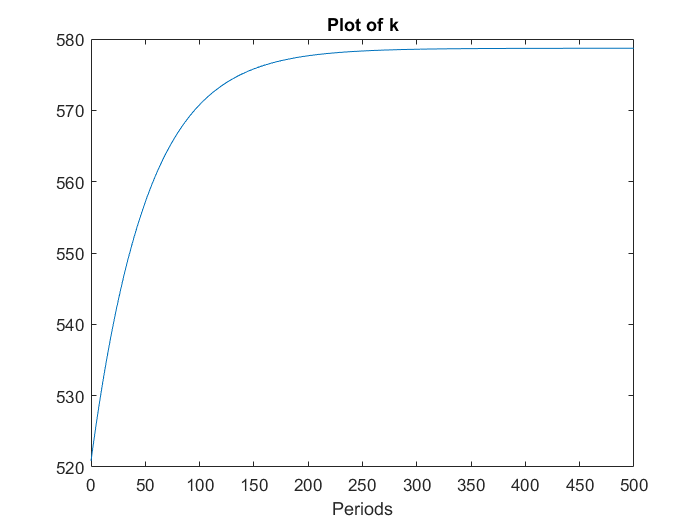
\includegraphics[width=8cm]{k-simulated.png}
\end{figure*}
\begin{figure*}[h!]
    \centering
    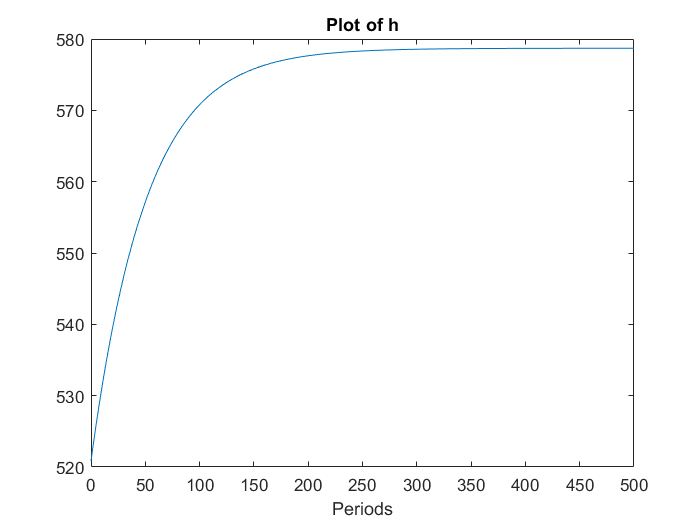
\includegraphics[width=8cm]{h-simulated.png}
\end{figure*}
\newpage
%%%%%%%%%%%%%%%%%%%%%%%%%%%%%%%%%%%%%%%%
%%%%%%%%%%%%%%%%%%%%%%%%%%%%%%%%%%%%%%%%
\end{document}